The equations of motion for a triaxial ellipsoid particle was first found by Jeffrey \cite{Jeffrey} but the first dimensionless equation for the Euler Angles was found by Yarin et al. \cite{Yarin} to be


\begin{subequations}\label{eq:jeffrey}
\begin{align}
\frac{d\theta}{dt} 	&= (g_2 \sin \psi + g_3 \cos \psi ) \sin \theta \\
\frac{d\phi}{dt} 	&= \tfrac{1}{2} + g_3\sin \psi - g_2 \cos \psi\\
\frac{d\psi}{dt}	&= g_1 + (g_2\cos \psi - g_3\sin \psi) \cos \theta \\
\end{align}
\end{subequations}

where the functions  $g_i$ are defined as

\begin{subequations}
\begin{align}
g_1 &= \frac{a_y^2 - a_z^2}{2(a_y^2 + a_z^2)} 
		\left(-\tfrac{1}{2}(\cos^2 \theta + 1 )\sin 2\phi \sin 2\psi + \cos\theta \cos 2\phi \cos 2\psi \right), \\
g_2 &= \frac{a_z^2 - a_x^2}{2(a_x^2 + a_z^2)}
		\left( -\cos\theta \sin 2\phi \sin\psi  +  \cos 2\phi \cos\psi \right), \\
g_3 &= \frac{a_x^2 - a_y^2}{2(a_x^2 + a_y^2)}
		\left( \cos\theta \sin 2\phi \cos\psi + \cos 2\phi \sin\psi \right)
\end{align}
\end{subequations}

where the angles are defined as can be seen in figure \ref{fig:eulerangles}

\begin{figure}
\begin{center}
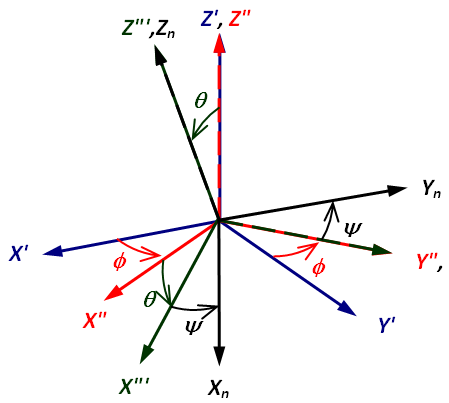
\includegraphics[width=0.7\textwidth]{figures/eulerangles.png}
\end{center}
\caption{}
\label{fig:eulerangles}
\end{figure}


%
%w = (f(t_0 + 2*pi*k) = f(t_0))/	N_rotations